\problemname{Around the Track}

\noindent
In order to compare race tracks, we wish to compute their lengths. A racetrack is strictly two-dimensional (no elevation). It is described by two simple polygons, where one is completely contained inside the other. The track is the region between these two polygons. We define the length of the track as the absolute minimum distance that one needs to travel in order to complete a lap. This could involve traveling on the very edge of the track and arbitrarily sharp cornering (see Figure~\ref{fig:racetrack:sample}).

\begin{figure}[h]
    \begin{center}
    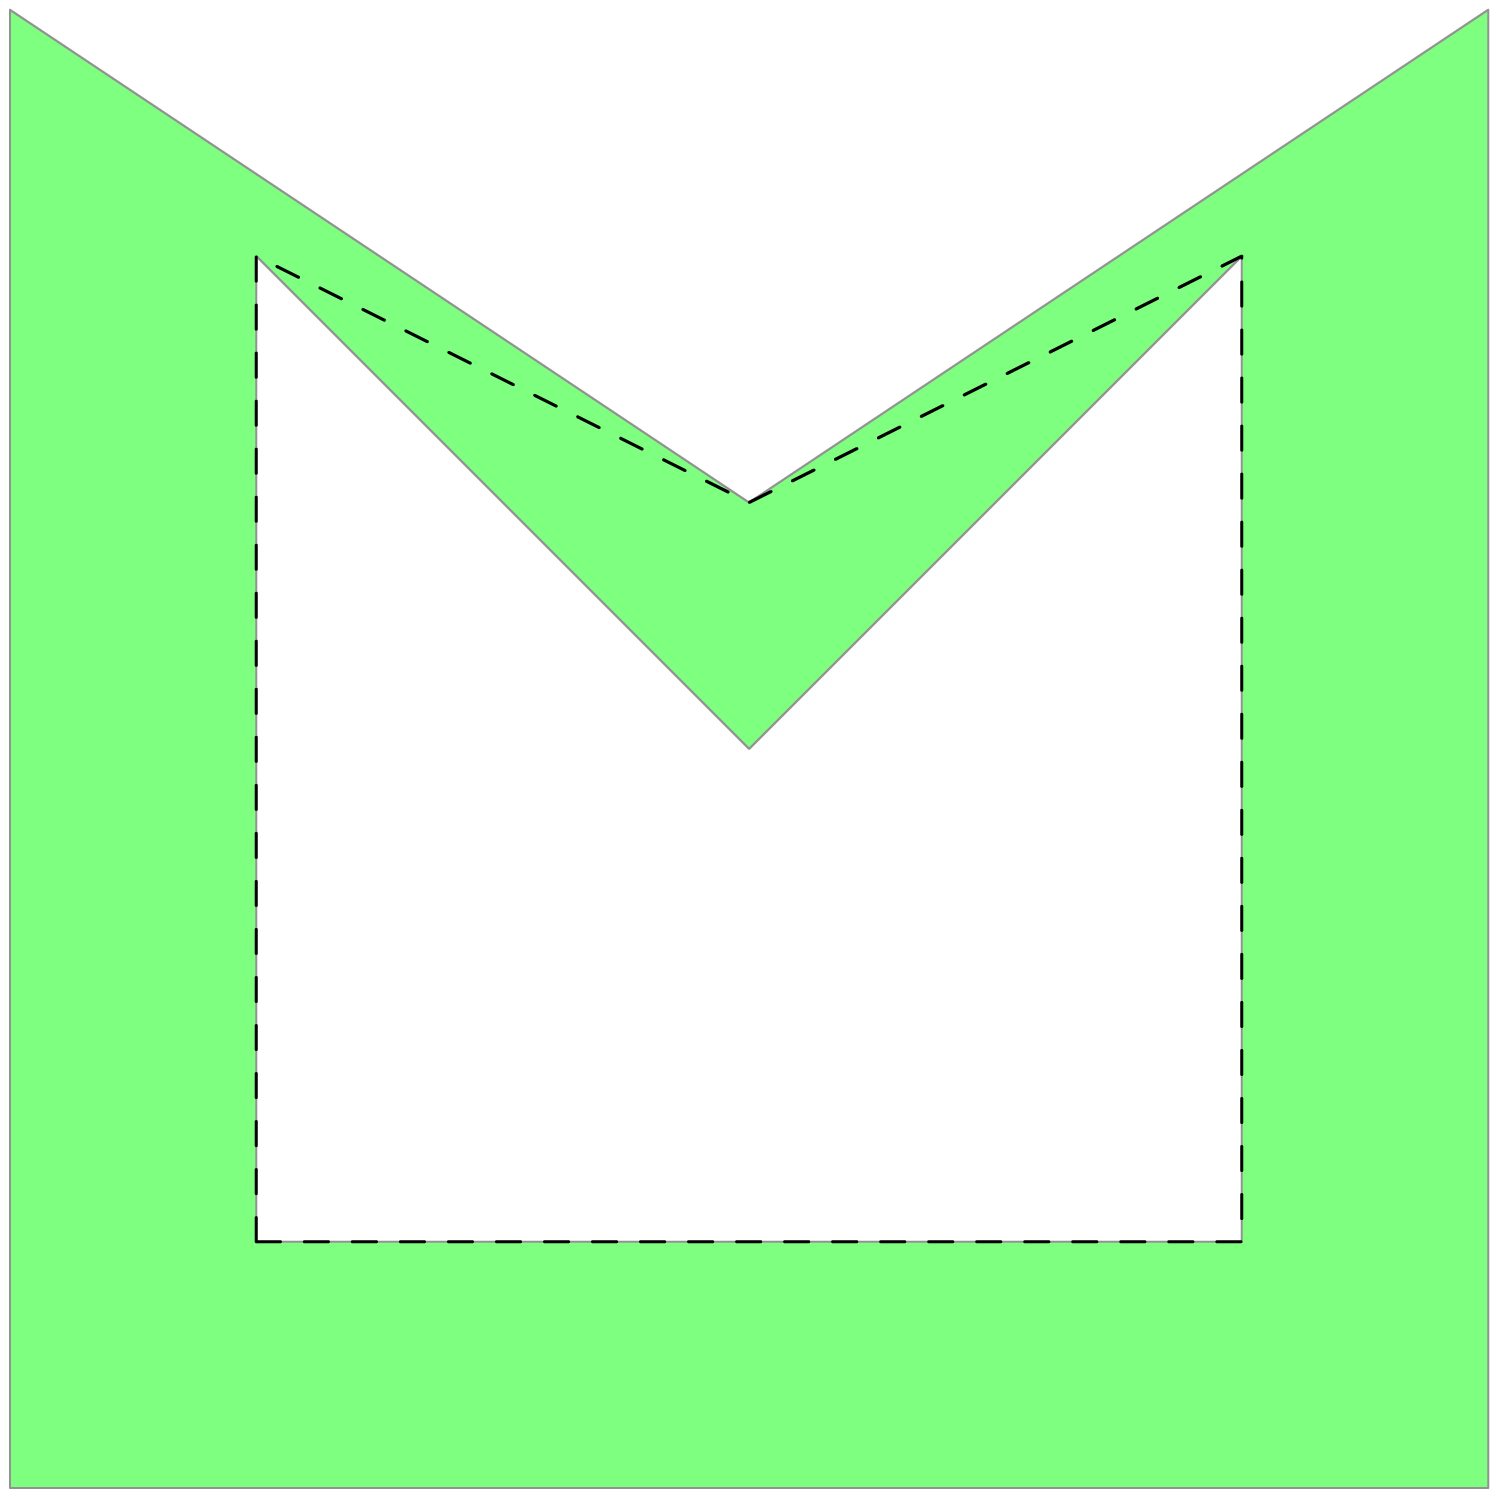
\includegraphics[width=0.3\textwidth]{racetrack-3}
    \caption{Illustration of sample input number 3 together with the shortest route around the track (dashed).}
    \label{fig:racetrack:sample}
    \end{center}
\end{figure}

\section*{Input}

The input consists of:
\begin{itemize}
  \item one line with one integer $n$ ($3 \leq n \leq 50$), the number of vertices of the inner polygon;
  \item $n$ lines, the $i$th of which contains two integers $x_i$ and $y_i$ ($ -5\,000 \leq x_i, y_i \leq 5\,000$): the coordinates of the $i$th vertex of the inner polygon;
  \item one line with one integer $m$ ($3 \leq m \leq 50$), the number of vertices of the outer polygon;
  \item $m$ lines, the $i$th of which contains two integers $x_i$ and $y_i$ ($ -5\,000 \leq x_i, y_i \leq 5\,000$): the coordinates of the $i$th vertex of the outer polygon.
\end{itemize}
For both polygons, the vertices are given in counterclockwise order. The borders of the two polygons do not intersect or touch each other.

\section*{Output}

Output one line with one floating point number: the length of the race
track.  Your answer should have an absolute or relative error of at most $10^{-6}$.
